% THIS IS SIGPROC-SP.TEX - VERSION 3.1
% WORKS WITH V3.2SP OF ACM_PROC_ARTICLE-SP.CLS
% APRIL 2009
%
% It is an example file showing how to use the 'acm_proc_article-sp.cls' V3.2SP
% LaTeX2e document class file for Conference Proceedings submissions.
% ----------------------------------------------------------------------------------------------------------------
% This .tex file (and associated .cls V3.2SP) *DOES NOT* produce:
%       1) The Permission Statement
%       2) The Conference (location) Info information
%       3) The Copyright Line with ACM data
%       4) Page numbering
% ---------------------------------------------------------------------------------------------------------------
% It is an example which *does* use the .bib file (from which the .bbl file
% is produced).
% REMEMBER HOWEVER: After having produced the .bbl file,
% and prior to final submission,
% you need to 'insert'  your .bbl file into your source .tex file so as to provide
% ONE 'self-contained' source file.
%
% Questions regarding SIGS should be sent to
% Adrienne Griscti ---> griscti@acm.org
%
% Questions/suggestions regarding the guidelines, .tex and .cls files, etc. to
% Gerald Murray ---> murray@hq.acm.org
%
% For tracking purposes - this is V3.1SP - APRIL 2009

\documentclass{acm_proc_article-sp}
\usepackage{listings}
\usepackage{graphicx}

\begin{document}

\title{Comparing and Contrasting {\ttlit Pattern Match} Algorithm Solutions}
\subtitle{Concentrating on Fast Matching and Tree Matching Techniques}

\numberofauthors{1} 
\author{
\alignauthor
Kwangju Kim\\
       \affaddr{Miami University Department of Computer Science and Software Engineering}\\
       \email{kimk3 (at) miamioh.edu}
}

\date{November 30, 2016}


\maketitle
\begin{abstract}
This paper investigates the two research papers discussing pattern match algorithm, one of the fundamental research field in the computer science. Two papers try to reduce the complexity of problem solution.
\end{abstract}

% % A category with the (minimum) three required fields
% \category{H.4}{Information Systems Applications}{Miscellaneous}
% %A category including the fourth, optional field follows...
% \category{D.2.8}{Software Engineering}{Metrics}[complexity measures, performance measures]

% \terms{Theory}

% \keywords{ACM proceedings, \LaTeX, text tagging} % NOT required for Proceedings

\section{Introduction}
\begin{flushleft}
Pattern matching techniques are widely used in the computer science studies. Few examples include formal language theory, compiler, artificial intelligence, searching algorithm, etc. The use of proper pattern matching will help develop the complex algorithm implementation with the few lines of actual code. However, it is imperative that the pattern matching will require the massive amount of resources and time. In order to resolve this drawback, many computer scientists had tried alternative method to beat the ordinary time and space complexity. 

There are many reasons the better pattern match algorithm is important. The main reason is, meanwhile, that with the better algorithm, the lighter code and faster sequence search can be accomplished, instead of using multiple loops for finding patterns in the literal sequence manually and getting penalized with respect of the time complexity. This is so vital in the area where the rapidity is necessary, for example, gene examination in bioinformatics, or stock market. The better pattern matching must be faster and/or more memory-space-efficient.
\end{flushleft}

\section{Manual, Brute Force Method}
\begin{figure}
\caption{Brute force, $naive$ method}
\begin{lstlisting}
function match(str, pattern) {
  result = 0; str_len = length(str);
  ptn_len = length(pattern);
  for (i = 0; i < str_len - ptn_len; i++) {
    flag = true;
    for (j = 0; j < ptn_len; j++) {
      if (str[j] != pattern[j]) {
        flag = false;
        break;
      }
    }
    if (flag) {
      result++;
    }
  }
  return result;
}
\end{lstlisting}
\end{figure}

\begin{flushleft}
The manual, 'brute force' method for pattern match is mostly looping several times to check each character value~\cite{Fast}. Generally, the double-nested for loop will be used to iterate both an original string literal and a pattern literal. The algorithm can be represented like the Figure 1. The algorithm introduced above is very ugly and inefficient pattern match method. In a worse case, the time complexity will rise to $O(n^2)$, even if it is confirmed that the certain character sequence interval does not match the given pattern.
\end{flushleft}

\section{Important Definitions}
\subsection{Terms}
\begin{flushleft}
In order to handle this problem, we have to define a set of terms to make what we should do more clear. A term \textit{pattern} stands for the regularity and/or similarity which two character sequences show. We will consider \textit{stirng literal} as an alias of the term \textit{character sequence}. In this problem, we will only investigate the pattern matching of the Roman alphabet characters in US-ASCII table.
\end{flushleft}

\subsection{Problem Space}
\begin{flushleft}
First of all, the main purpose of investigating the better pattern match algorithm problems is reducing the complexity. It is really important because the better pattern match solution should have better complexity than manual search method shown above.

The final goal of this algorithm is to find the efficient way to accomplish pattern matching. We use the string literals to perform pattern match, and regular expressions which defines the pattern. Then we want to get returned the number of pattern that matches, and/or desired substring from the string literal which corresponds the pattern.
\end{flushleft}

% Citation of Einstein paper~\cite{Einstein} ~\cite{Test}.
\section{Discussion of Solutions}
\subsection{Fast Pattern Match}
\begin{flushleft}
Fast pattern match algorithm introduces the way to reduce the pattern match time complexity to the sum of both the length of pattern and the length of the target string literal~\cite{Fast}. The main idea of this algorithm is compiling the pattern as well as using an additional table, for example, 'next'. The author insists the method should be faster because the algorithm must make cases for all indexes of a given character sequence. The subject pattern will have several switch statements which expedites the process. The average complexity possible will be $O(m + n)$, where $m$ is the size of pattern and $n$ is one of the target string literal.

The pseudocode is described in Figure 2, directly extracted from the paper.
\end{flushleft}

\begin{figure}
  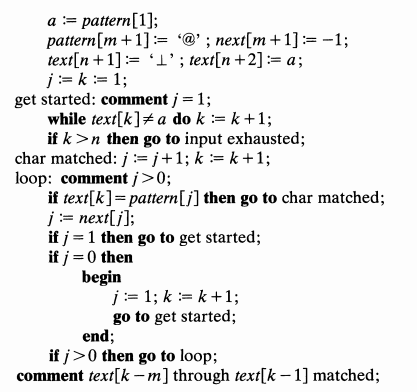
\includegraphics[scale=.7]{fastpattern01}
  \caption{Basic Idea of Fast Match Algorithm~\cite{Fast}}
\end{figure}

\subsection{Tree Pattern Match}
\begin{flushleft}
Unlike the fast pattern match, tree pattern match utilizes a tree structure to perform a pattern match~\cite{Tree}. The goal of this method is to reduce the complexity which bounds to the linear function with respect to either the size of pattern, or the size of the tree structure called a \textit{subject tree}~\cite{Tree}. The major implementation of their algorithm is using a tree structure to solve the problem. The method will use the constructed tree structure to perform a pattern matching. The authors suggest two submethods to approach this algorithm; one is the top-down, the other is the bottom-up. They first constructed the top-down method, and then traced the bottom-up method.

The authors' pseudocode is shared and shown in Figure 3, directly extracted from the paper.
\end{flushleft}

\begin{figure}
  \caption{Pseudocode of Tree Matching~\cite{Tree}}
  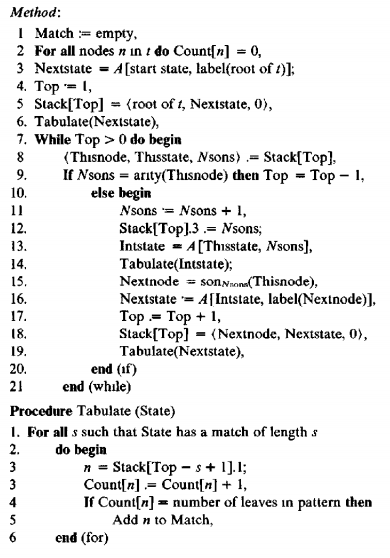
\includegraphics[scale=.7]{treematch02}
\end{figure}

\section{Traits}
\begin{flushleft}
Two pattern match algorithm introduced above have few traits to focus in.
\end{flushleft}

\subsection{Possible Drawbacks}
\begin{flushleft}
Meanwhile the two papers introduced the innovative way of pattern matching, both methods have a common drawback which require a preprocessing. A fast pattern match require a precompiled pattern to expedite the process; without it, the complexity will not be different from \textit{naive} ones. A tree pattern match requires the worst case $O(n)$ time for tree construction, which is basically the worst case of a binary tree. Since preprocessing requires $O(n)$ generally, the worst case will not have a major difference with the original $naive$ method(s).
\end{flushleft}

\subsection{Strings Which Cannot Solve in Linear Time Complexity}
\begin{flushleft}
Some of the strings cannot be solved in a linear time complexity using the algorithms shown above. For example, fast pattern match shows a dramatic time complexity increase when the target string is a palindrome~\cite{Fast}. The authors noted that handling palindrome is still being investigated by computer scientists which is not being solved until now~\cite{Fast}. It is important because if we can handle the palindrome easily, we can reduce the complexity by $O(n/2)$, omitting the second half because the sequence should be the same.
\end{flushleft}

\section{Acknowledgement}
\begin{flushleft}
I share a special thank to Dr. John Femiani for instructing Algorithm course this fall.
\end{flushleft}

\bibliographystyle{abbrv}
\bibliography{sample}

%\balancecolumns 

\end{document}
